% Drawing 156-9/02-1 -- folder 156-9, batch 02, archive page 31 (PDF page 32).
% Transcription: un triangle de sommets $a$ (en haut), $b$, $c$ ; la moitié gauche hachurée, un segment de $a$ au point $d$, marqué d'un gros point, sur le côté $[b,c]$.
% Kind: triangle with a cevian. Method 2 (schematic redraw from the facsimile). Status: ok.
% Notes: Triangle a (top), b, c; the left half hatched; a segment from a to the point d, marked by a big dot, on the side [b, c].
% Coordinates: 1 unit = 1 mm = 1/100 of the crop width (bbox in page fractions: [0.3, 0.73, 0.48, 0.82]).
% Redrawn by Claude (claude-opus-5-5), issue #73, 2026-11-07; not checked by a human; not compiled (no TeX in the session).
% Rights: reproduces part of the work -- behind RENDER_TRANSCRIPTS, never published by itself.
\documentclass[tikz,border=3pt]{standalone}
\usepackage{amsmath,amssymb}
\usetikzlibrary{patterns,arrows.meta}
\tikzset{pencil/.style={black!45}, struck/.style={black!35}, mark/.style={circle,draw,inner sep=1.3pt}, pt/.style={circle,fill,inner sep=0.9pt}, opt/.style={circle,draw,fill=white,inner sep=1.1pt}}
\begin{document}
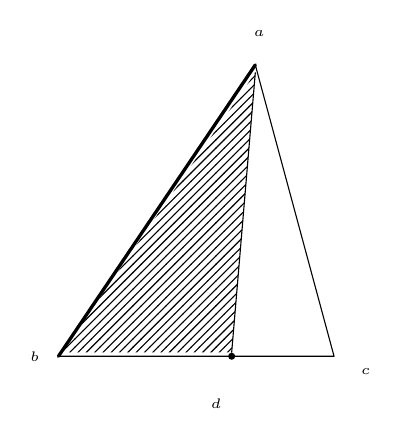
\begin{tikzpicture}[x=1mm,y=1mm,line cap=round,line join=round,font=\scriptsize]
\draw (73,-16) -- (48,-53) -- (83,-53) -- cycle;
\draw (73,-17) -- (70,-52.5);
\fill[pattern=north east lines] (73,-17) -- (48.5,-52.5) -- (70,-52.5) -- cycle;
\draw[very thick] (73,-16) -- (48,-53);
\node[pt] at (70,-53) {};
\node[inner sep=1pt] at (73.5,-12) {\tiny $a$};
\node[inner sep=1pt] at (45,-53) {\tiny $b$};
\node[inner sep=1pt] at (87,-55) {\tiny $c$};
\node[inner sep=1pt] at (68,-59) {\tiny $d$};
\end{tikzpicture}
\end{document}
